\documentclass{standalone}
\usepackage{tikz}
\usetikzlibrary{patterns, positioning}
\usepackage[sfdefault]{ClearSans} %% option 'sfdefault' activates Clear Sans as the default text font
\usepackage[T1]{fontenc}

\begin{document}
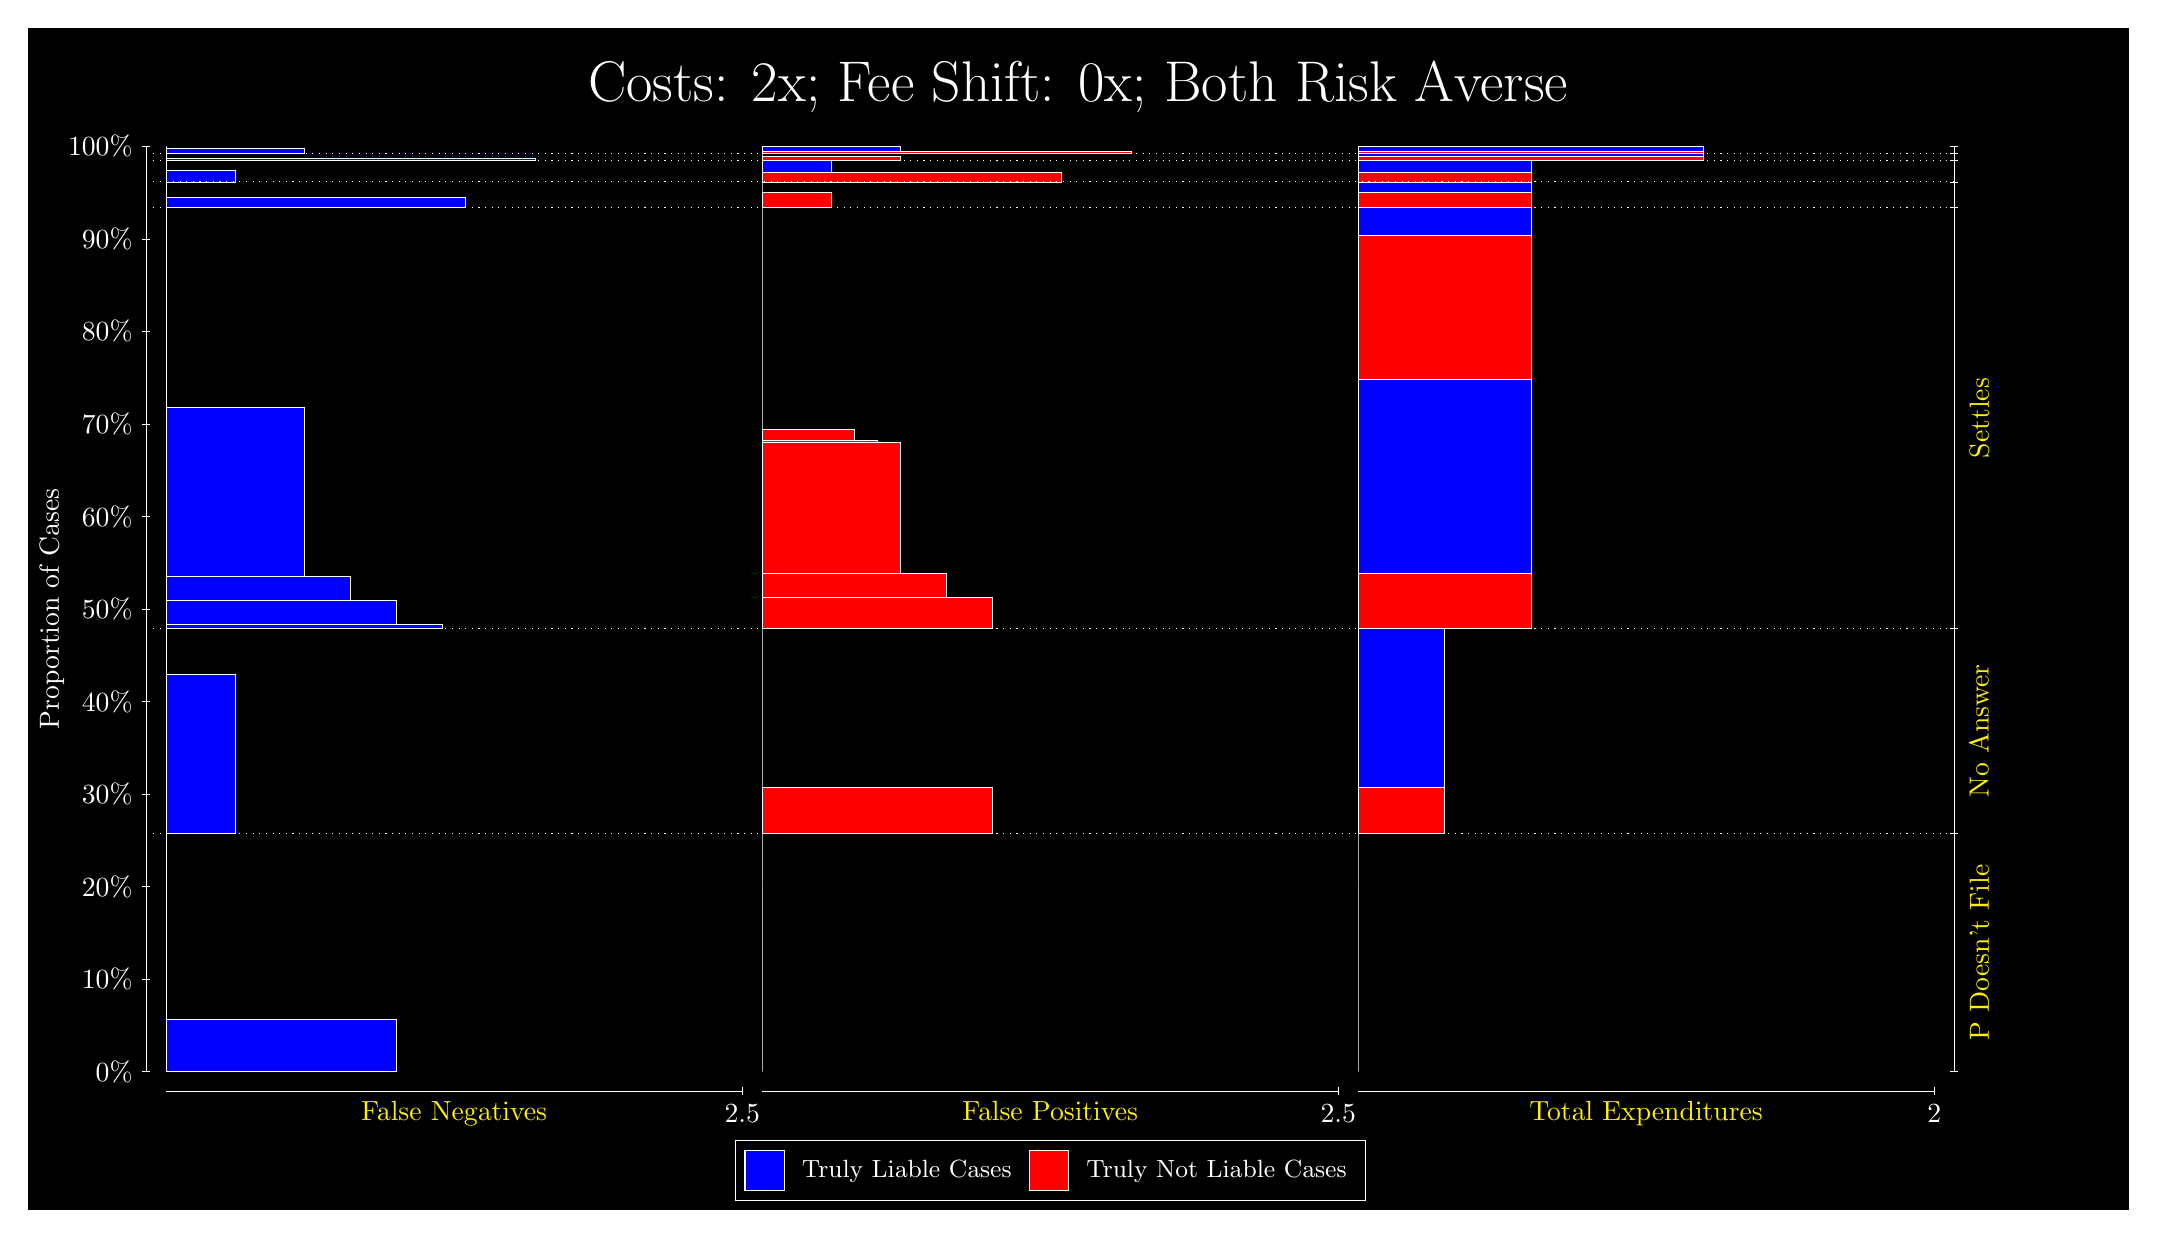
\begin{tikzpicture}
\draw[fill=black] (0,0) rectangle (26.667,15);
\draw[text=white] (0,13.5) rectangle (26.667,15) node[midway] {\huge Costs: 2x; Fee Shift: 0x; Both Risk Averse};
\draw[white, very thin] (1.5,1.75) -- (1.5,13.5);
\node[rotate=90, text=white, anchor=center] at (0.3, 7.625) {Proportion of Cases};
\draw[white, very thin] (1.45,1.75) -- (1.55,1.75);
\node[text=white, anchor=east] at (1.45, 1.75) {0\%};
\draw[white, very thin] (1.45,2.925) -- (1.55,2.925);
\node[text=white, anchor=east] at (1.45, 2.925) {10\%};
\draw[white, very thin] (1.45,4.1) -- (1.55,4.1);
\node[text=white, anchor=east] at (1.45, 4.1) {20\%};
\draw[white, very thin] (1.45,5.275) -- (1.55,5.275);
\node[text=white, anchor=east] at (1.45, 5.275) {30\%};
\draw[white, very thin] (1.45,6.45) -- (1.55,6.45);
\node[text=white, anchor=east] at (1.45, 6.45) {40\%};
\draw[white, very thin] (1.45,7.625) -- (1.55,7.625);
\node[text=white, anchor=east] at (1.45, 7.625) {50\%};
\draw[white, very thin] (1.45,8.8) -- (1.55,8.8);
\node[text=white, anchor=east] at (1.45, 8.8) {60\%};
\draw[white, very thin] (1.45,9.975) -- (1.55,9.975);
\node[text=white, anchor=east] at (1.45, 9.975) {70\%};
\draw[white, very thin] (1.45,11.15) -- (1.55,11.15);
\node[text=white, anchor=east] at (1.45, 11.15) {80\%};
\draw[white, very thin] (1.45,12.325) -- (1.55,12.325);
\node[text=white, anchor=east] at (1.45, 12.325) {90\%};
\draw[white, very thin] (1.45,13.5) -- (1.55,13.5);
\node[text=white, anchor=east] at (1.45, 13.5) {100\%};

\draw[white, very thin] (24.457,1.75) -- (24.457,13.5);
\draw[white, very thin] (24.407,1.75) -- (24.507,1.75);
\node[anchor=west] at (24.407, 1.75) {};
\draw[white, very thin] (24.407,4.7744) -- (24.507,4.7744);
\node[anchor=west] at (24.407, 4.7744) {};
\draw[white, very thin] (24.407,7.3782) -- (24.507,7.3782);
\node[anchor=west] at (24.407, 7.3782) {};
\draw[white, very thin] (24.407,12.722) -- (24.507,12.722);
\node[anchor=west] at (24.407, 12.722) {};
\draw[white, very thin] (24.407,13.049) -- (24.507,13.049);
\node[anchor=west] at (24.407, 13.049) {};
\draw[white, very thin] (24.407,13.317) -- (24.507,13.317);
\node[anchor=west] at (24.407, 13.317) {};
\draw[white, very thin] (24.407,13.408) -- (24.507,13.408);
\node[anchor=west] at (24.407, 13.408) {};
\draw[white, very thin] (24.407,13.5) -- (24.507,13.5);
\node[anchor=west] at (24.407, 13.5) {};

\draw[white, very thin, fill=blue] (1.75,1.75) rectangle (4.6775,2.4138);
\draw[white, very thin, fill=red] (1.75,2.4138) rectangle (1.75,4.7744);
\draw[white, very thin, fill=blue] (1.75,4.7744) rectangle (2.6283,6.7985);
\draw[white, very thin, fill=red] (1.75,6.7985) rectangle (1.75,7.3782);
\draw[white, very thin, fill=blue] (1.75,7.3782) rectangle (5.2631,7.4241);
\draw[white, very thin, fill=blue] (1.75,7.4241) rectangle (4.9703,7.4309);
\draw[white, very thin, fill=blue] (1.75,7.4309) rectangle (4.6775,7.7307);
\draw[white, very thin, fill=blue] (1.75,7.7307) rectangle (4.092,8.0351);
\draw[white, very thin, fill=blue] (1.75,8.0351) rectangle (3.5065,10.191);
\draw[white, very thin, fill=red] (1.75,10.191) rectangle (1.75,12.722);
\draw[white, very thin, fill=blue] (1.75,12.722) rectangle (5.5558,12.853);
\draw[white, very thin, fill=red] (1.75,12.853) rectangle (1.75,13.049);
\draw[white, very thin, fill=blue] (1.75,13.049) rectangle (2.6283,13.2);
\draw[white, very thin, fill=red] (1.75,13.2) rectangle (1.75,13.317);
\draw[white, very thin, fill=blue] (1.75,13.317) rectangle (6.4341,13.346);
\draw[white, very thin, fill=red] (1.75,13.346) rectangle (1.75,13.408);
\draw[white, very thin, fill=blue] (1.75,13.408) rectangle (3.5065,13.471);
\draw[white, very thin, fill=red] (1.75,13.471) rectangle (1.75,13.5);
\draw[white, very thin, fill=red] (9.3189,1.75) rectangle (9.3189,4.1106);
\draw[white, very thin, fill=blue] (9.3189,4.1106) rectangle (9.3189,4.7744);
\draw[white, very thin, fill=red] (9.3189,4.7744) rectangle (12.246,5.3541);
\draw[white, very thin, fill=blue] (9.3189,5.3541) rectangle (9.3189,7.3782);
\draw[white, very thin, fill=red] (9.3189,7.3782) rectangle (12.246,7.7718);
\draw[white, very thin, fill=red] (9.3189,7.7718) rectangle (11.661,8.0762);
\draw[white, very thin, fill=red] (9.3189,8.0762) rectangle (11.075,9.7417);
\draw[white, very thin, fill=red] (9.3189,9.7417) rectangle (10.783,9.7615);
\draw[white, very thin, fill=red] (9.3189,9.7615) rectangle (10.49,9.9092);
\draw[white, very thin, fill=blue] (9.3189,9.9092) rectangle (9.3189,12.722);
\draw[white, very thin, fill=red] (9.3189,12.722) rectangle (10.197,12.918);
\draw[white, very thin, fill=blue] (9.3189,12.918) rectangle (9.3189,13.049);
\draw[white, very thin, fill=red] (9.3189,13.049) rectangle (13.125,13.166);
\draw[white, very thin, fill=blue] (9.3189,13.166) rectangle (10.197,13.317);
\draw[white, very thin, fill=red] (9.3189,13.317) rectangle (11.075,13.379);
\draw[white, very thin, fill=blue] (9.3189,13.379) rectangle (9.3189,13.408);
\draw[white, very thin, fill=red] (9.3189,13.408) rectangle (14.003,13.436);
\draw[white, very thin, fill=blue] (9.3189,13.436) rectangle (11.075,13.5);
\draw[white, very thin, fill=red] (16.888,1.75) rectangle (16.888,4.1106);
\draw[white, very thin, fill=blue] (16.888,4.1106) rectangle (16.888,4.7744);
\draw[white, very thin, fill=red] (16.888,4.7744) rectangle (17.986,5.3541);
\draw[white, very thin, fill=blue] (16.888,5.3541) rectangle (17.986,7.3782);
\draw[white, very thin, fill=red] (16.888,7.3782) rectangle (19.083,8.0762);
\draw[white, very thin, fill=blue] (16.888,8.0762) rectangle (19.083,10.537);
\draw[white, very thin, fill=red] (16.888,10.537) rectangle (19.083,12.37);
\draw[white, very thin, fill=blue] (16.888,12.37) rectangle (19.083,12.722);
\draw[white, very thin, fill=red] (16.888,12.722) rectangle (19.083,12.918);
\draw[white, very thin, fill=blue] (16.888,12.918) rectangle (19.083,13.049);
\draw[white, very thin, fill=red] (16.888,13.049) rectangle (19.083,13.166);
\draw[white, very thin, fill=blue] (16.888,13.166) rectangle (19.083,13.317);
\draw[white, very thin, fill=red] (16.888,13.317) rectangle (21.279,13.379);
\draw[white, very thin, fill=blue] (16.888,13.379) rectangle (21.279,13.408);
\draw[white, very thin, fill=red] (16.888,13.408) rectangle (21.279,13.436);
\draw[white, very thin, fill=blue] (16.888,13.436) rectangle (21.279,13.5);
\draw[white, dotted] (1.5,4.7744) -- (24.457,4.7744);
\draw[white, dotted] (1.5,7.3782) -- (24.457,7.3782);
\draw[white, dotted] (1.5,12.722) -- (24.457,12.722);
\draw[white, dotted] (1.5,13.049) -- (24.457,13.049);
\draw[white, dotted] (1.5,13.317) -- (24.457,13.317);
\draw[white, dotted] (1.5,13.408) -- (24.457,13.408);
\draw[white, very thin] (1.75,1.5) -- (9.0689,1.5);
\node[text=yellow, anchor=north] at (5.4094, 1.5) {False Negatives};
\draw[white, very thin] (9.0689,1.45) -- (9.0689,1.55);
\node[text=white, anchor=north] at (9.0689, 1.45) {2.5};

\draw[white, very thin] (9.3189,1.5) -- (16.638,1.5);
\node[text=yellow, anchor=north] at (12.978, 1.5) {False Positives};
\draw[white, very thin] (16.638,1.45) -- (16.638,1.55);
\node[text=white, anchor=north] at (16.638, 1.45) {2.5};

\draw[white, very thin] (16.888,1.5) -- (24.207,1.5);
\node[text=yellow, anchor=north] at (20.547, 1.5) {Total Expenditures};
\draw[white, very thin] (24.207,1.45) -- (24.207,1.55);
\node[text=white, anchor=north] at (24.207, 1.45) {2};

\node[text=yellow, centered, rotate=90] at (24.777, 3.2622) {P Doesn't File};
\node[text=yellow, centered, rotate=90] at (24.777, 6.0763) {No Answer};
\node[text=yellow, centered, rotate=90] at (24.777, 10.05) {Settles};





\draw (12.978300999999998,1.5) node[draw=none] (baseCoordinate) {};
\begin{scope}[align=center]
        \matrix[scale=0.5, draw=white, below=0.5cm of baseCoordinate, nodes={draw}, column sep=0.1cm]{
            \node[rectangle, draw, minimum width=0.5cm, minimum height=0.5cm, fill=blue] {}; &
            \node[draw=none, font=\small, text=white] (B) {Truly Liable Cases}; &
            \node[rectangle, draw, minimum width=0.5cm, minimum height=0.5cm, fill=red] {}; &
            \node[draw=none, font=\small, text=white] (B) {Truly Not Liable Cases}; \\
            };
\end{scope}

\end{tikzpicture}
\end{document}